%% 
%% Copyright 2007-2020 Elsevier Ltd
%% 
%% This file is part of the 'Elsarticle Bundle'.
%% ---------------------------------------------
%% 
%% It may be distributed under the conditions of the LaTeX Project Public
%% License, either version 1.2 of this license or (at your option) any
%% later version.  The latest version of this license is in
%%    http://www.latex-project.org/lppl.txt
%% and version 1.2 or later is part of all distributions of LaTeX
%% version 1999/12/01 or later.
%% 
%% The list of all files belonging to the 'Elsarticle Bundle' is
%% given in the file `manifest.txt'.
%% 

%% Template article for Elsevier's document class `elsarticle'
%% with numbered style bibliographic references
%% SP 2008/03/01
%%
%% 
%%
%% $Id: elsarticle-template-num.tex 190 2020-11-23 11:12:32Z rishi $
%%
%%
\documentclass[preprint,5p,twocolumn]{elsarticle}

\usepackage{amsmath,amssymb,amsfonts,amsthm}
\usepackage{algorithmic}
\usepackage{graphicx}
\usepackage{textcomp}
\usepackage{xcolor}
\usepackage{pifont}
\newtheorem{theorem}{Theorem}
\newtheorem{lemma}[theorem]{Lemma}
\newtheorem{definition}[theorem]{Definition}

%% Use the option review to obtain double line spacing
%% \documentclass[authoryear,preprint,review,12pt]{elsarticle}

%% Use the options 1p,twocolumn; 3p; 3p,twocolumn; 5p; or 5p,twocolumn
%% for a journal layout:
%% \documentclass[final,1p,times]{elsarticle}
%% \documentclass[final,1p,times,twocolumn]{elsarticle}
%% \documentclass[final,3p,times]{elsarticle}
%% \documentclass[final,3p,times,twocolumn]{elsarticle}
%% \documentclass[final,5p,times]{elsarticle}
%% \documentclass[final,5p,times,twocolumn]{elsarticle}

%% For including figures, graphicx.sty has been loaded in
%% elsarticle.cls. If you prefer to use the old commands
%% please give \usepackage{epsfig}

%% The amssymb package provides various useful mathematical symbols
\usepackage{amssymb}

%% The amsthm package provides extended theorem environments
%% \usepackage{amsthm}

%% The lineno packages adds line numbers. Start line numbering with
%% \begin{linenumbers}, end it with \end{linenumbers}. Or switch it on
%% for the whole article with \linenumbers.
%% \usepackage{lineno}

\journal{Information Processing Letters}

\begin{document}

\begin{frontmatter}

%% Title, authors and addresses

%% use the tnoteref command within \title for footnotes;
%% use the tnotetext command for theassociated footnote;
%% use the fnref command within \author or \address for footnotes;
%% use the fntext command for theassociated footnote;
%% use the corref command within \author for corresponding author footnotes;
%% use the cortext command for theassociated footnote;
%% use the ead command for the email address,
%% and the form \ead[url] for the home page:
%% \title{Title\tnoteref{label1}}
%% \tnotetext[label1]{}
%% \author{Name\corref{cor1}\fnref{label2}}
%% \ead{email address}
%% \ead[url]{home page}
%% \fntext[label2]{}
%% \cortext[cor1]{}
%% \affiliation{organization={},
%%             addressline={},
%%             city={},
%%             postcode={},
%%             state={},
%%             country={}}
%% \fntext[label3]{}

\title{Interactive Non-Interference Does Not (Always) Compose}

%% use optional labels to link authors explicitly to addresses:
%% \author[label1,label2]{}
%% \affiliation[label1]{organization={},
%%             addressline={},
%%             city={},
%%             postcode={},
%%             state={},
%%             country={}}
%%
%% \affiliation[label2]{organization={},
%%             addressline={},
%%             city={},
%%             postcode={},
%%             state={},
%%             country={}}

\author[inst1]{François Hublet}

\affiliation[inst1]{organization={ETH Zürich},%Department and Organization
            addressline={CNB F 107.2, Universitätstrasse 6},
            city={Zürich},
            postcode={8051},
            country={Switzerland}}
\begin{abstract}
  We study the notion of Interactive Non-Interference (INI) as introduced by
  O'Neill et al.~\cite{ONeill2006} and Rafnsson et al.~\cite{Rafnsson2012}.
  We show that, unlike claimed in previous work, INI is generally not compositional when
  programs are non-deterministic. To this end, we exhibit elementary attacks on INI that cover
  both blocking and non-blocking communication between interactive programs. Then, we
  prove that compositionality does indeed hold when we require programs to be deterministic.    
\end{abstract}

%%Graphical abstract
%\begin{graphicalabstract}
%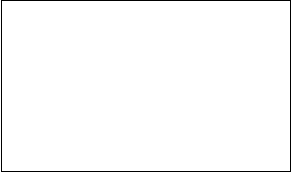
\includegraphics{grabs}
%\end{graphicalabstract}

%%Research highlights
%\begin{highlights}
%\item Research highlight 1
%\item Research highlight 2
%\end{highlights}

\begin{keyword}
%% keywords here, in the form: keyword \sep keyword
keyword one \sep keyword two
%% PACS codes here, in the form: \PACS code \sep code
\PACS 0000 \sep 1111
%% MSC codes here, in the form: \MSC code \sep code
%% or \MSC[2008] code \sep code (2000 is the default)
\MSC 0000 \sep 1111
\end{keyword}

\end{frontmatter}

%% \linenumbers

%% main text
\newcommand{\xmark}{{\color{red}\ding{55}}}%
%\definecolor{darkgreen}{rgb}{0.13, 0.55, 0.13}
\newcommand{\cmark}{{\color{darkgreen}\checkmark}}%


\newcommand{\sA}{s_{\mathtt{A}}}
\newcommand{\sB}{s_{\mathtt{B}}}
\newcommand{\sC}{s_{\mathtt{C}}}
\newcommand{\sD}{s_{\mathtt{D}}}
\newcommand{\sE}{s_{\mathtt{E}}}
\newcommand{\sF}{s_{\mathtt{F}}}
\newcommand{\PA}{P_{\mathtt{A}}}
\newcommand{\PB}{P_{\mathtt{B}}}
\newcommand{\PC}{P_{\mathtt{C}}}
\newcommand{\pOut}[2]{\mathtt{out}_{#1}(#2)}
\newcommand{\pIn}[2]{\mathtt{in}_{#1}(#2)}
\newcommand{\pAssign}[2]{#1 := #2}
\newcommand{\pComp}[2]{#1 \mid #2}
\newcommand{\Lattice}{\mathcal{L}}
\renewcommand{\doteq}{\overset{.}{=}}


% TODO: Randomness vs. Nondeterminism
\section{Introduction}

\emph{Interactive programs} were introduced by O'Neill, Clarkson, and Chong~\cite{ONeill2006} as a model
for imperative programs that interact with users through inputs and outputs while updating
their state. With interactive programs, users can adapt their outputs depending on previously
seen inputs in a malicious way, which poses specific challenges for information-flow control.
To illustrate these challenges, O'Neill et al.~\cite{ONeill2006} use a program
similar to the following, where $\mid$ denotes non-deterministic choice and $\oplus$ stands for `exclusive or':
\begin{align*}
  P_0=~&(\pComp{\pAssign{x}{0}}{\pAssign{x}{1}});\\
  &\pOut{H}{x};\\
  &\pIn{H}{y};\\
  &\pOut{L}{x \oplus y}.
\end{align*}
At first glance, program $P_0$ does not seem to propagate information from high to low channels, as
the high information input from channel $H$ is \emph{xor}ed with the random value in $x$ before being
output to $L$. However, attacks become possible when interaction is considered. Suppose that Hillary,
who can read and write on channel $H$, wants to send a bit of information $b$ to Hillary, who can read
on channel $L$. Hillary can simply observe the bit $x$ and set $y$ to $b \oplus x$; then Laura will read
$x \oplus y = x \oplus (b \oplus x) = b$ on $L$, which is exactly the bit Hillary wanted to transmit.

To guarantee that no information flows from high to low channels in interactive programs, the notion
of interactive noninterference~\cite{ONeill2006} (INI) has been introduced. INI relies on \emph{strategies}
that encode how users with different clearance levels provide new inputs depending on the outputs
they have been able to observe up to the present. In the above example, INI is violated because
there exist two strategies differing only on high channels (the one where Hillary wants to transmit $1$ and the one
where Hillary wants to transmit $0$) that must produce different outputs on low channels.

This initial study on interactive programs has given rise to a number of follow-ups works.
Clark and Hunt~\cite{Clark2008} have shown that, in the case of \emph{deterministic} interactive
programs, considering general strategies was not needed. They showed that those programs satisfying INI
where exactly those satisfying nonintereference for \emph{stream strategies} where the sequence of user
inputs is set ahead of time independently of the program's outputs. Later, Rafnsson, Hedin, and Sabelfeld
reconsidered the general case~\cite{Rafnsson2012}, revisiting it in two different directions. First, they
extended O'Neill et al.'s model to support \emph{non-total} strategies in which channels may not always
contain data ready to be input, and for which the \emph{presence} and \emph{value} on data transmitted on
channels may have different security levels. In their model, a channel has levels, e.g., $H^L$, if the
presence of an input on it is public, but the value of the input is private. When a program tries to perform
an input on a channel that contains no input, the execution is blocked, which may induce a new information
channel. Second, Rafnsson et al. studied the composition of INI. They claimed that INI on their two-level model
was compositional for both deterministic and non-deterministic programs, and provided a type system to statically
check in INI in imperative programs.

For interactive non-interference to be useful in real-world software systems, compositionality is arguably
a key property. Indeed, most privacy-sensitive systems that interact with users especially in the web
are component-based, e.g., because they are multi-tier or run on a microservice architecture.
In general, being able to check non-interference component-wise rather than globally results in a significant
decrease in complexity and strong modularity benefits.
Even more critically, it might be the only practical approach when dealing with systems that
combine components from multiple code providers that may not be willing to share their sources.

Unfortunately, and as we will show in the first part of this paper, the compositionality property claimed
by Rafnsson et al. for INI~\cite[Theorem V.1]{Rafnsson2012} does not hold for general programs. Attacks against
INI exist for non-deterministic programs in both Rafnsson et al.'s non-total (blocking) setup and the original
total (non-blocking) setup by O'Neill et al.~\cite{ONeill2006}, who did not make any compositionality claims.
The compositionality proofs provided in the original paper~\cite{Rafnsson2012} as well as three other related
publications~\cite{Rafnsson2014,Greiner2016,Greiner2018} are flawed. However, we show that the compositionality of INI
can be recovered for deterministic programs.

After reviewing interactive noninterference as introduced by O'Neill et al. and Rafnsson et al.~\cite{ONeill2006,Rafnsson2012}
(Section~\ref{sec:preliminaries}), we make the following contributions:
\begin{itemize}
\item We show that INI is non-compositional in both total and non-total setups by exhibiting elementary
  attacks. We also briefly review the flawed proofs presented in previous work and identify the mistakes they contain.
  (Section~\ref{sec:non-compositionality})
\item We show that INI is compositional when all programs are deterministic (Section~\ref{sec:deterministic}).
\end{itemize}

\section{Interactive Non-Interference}

\label{sec:preliminaries}

\newcommand{\Strat}{\mathbf{Strat}}
\newcommand{\StratNI}{\mathbf{Strat}\text{-}\mathrm{NI}}
\newcommand{\StratNINI}{\mathbf{Strat}\text{-}\mathrm{NINI}}
\newcommand{\StratTNI}{\mathbf{Strat}_\mathrm{T}\text{-}\mathrm{NI}}
\section{Non-compositionality}

\label{sec:non-compositionality}

In this section, we first show that the compositionality result claimed by Rafnsson, Hedin, and Sabelfeld
~\cite[Theorem V.1]{Rafnsson2012} does not hold. We then briefly discuss the flaws found in previously published proofs
of compositionality. Finally, we show how to extend our attack to the total setup originally considered by O'Neill et
al.~\cite{ONeill2006}.

\subsection{Non-compositionality for non-total strategies}

Our counterexample to the compositionality of INI is based on the following variant of a secret sharing~\cite{Shamir1979} protocol
for two parties. The proof is as follows:

\begin{theorem}[Non-compositionality]
  There exists $\sA, \sB \in \StratNI$ such that $\sA \parallel \sB \notin \StratNI$.
\end{theorem}
\begin{proof}
  Let $(\Lattice, \sqsubseteq)$ be the lattice with $\Lattice = \lbrace L, H, H_1, H_2, H_3 \rbrace$
  and $\sqsubseteq = \lbrace (L, \ell) \mid \ell \in \Lattice\rbrace \cup \lbrace (\ell, \ell) \mid \ell \in \Lattice\rbrace$, i.e.,
  all $H_i$-levels are incomparable and $L$ is lower than the $H_i$.

  We reuse the elements of $\Lattice$ as channel names and set
  $\forall \ell.~\gamma(\ell) = \ell^L$, thus giving all channels a low presence label.
  
  Consider the following programs $\PA$ and $\PB$ and states $\sA$ and $\sB$, where
  $\oplus$ denotes exclusive or and all variables are boolean:
  \begin{align*}
    \PA =~& \pIn{H}{r}; & \PB =~ & (\pComp{\pAssign{x'}{0}}{\pAssign{x'}{1}}); \\
        &(\pComp{\pAssign{x}{0}}{\pAssign{x}{1}}); && \pOut{H_2}{\neg x'};\\
        &\pOut{H_1}{\neg x}; && \pIn{H_1}{y'}; \\
        & \pIn{H_2}{y}; && \pOut{H_3}{x' \oplus y'} \\
          & \pOut{H_3}{r \oplus x \oplus y} \\
    \sA =~& \lbrace r = 0, x = 0, y = 0\rbrace & \sB =~& \lbrace x' = 0, y' = 0\rbrace.
  \end{align*}

  We first show that $\sA \in \StratNI$.

  Let $\ell \in \Lattice$, $\omega_1, \omega_2 \in \Strat$, and $t$ such that $\omega_1 =_\ell \omega_2$
  and $\omega_1 \vDash s \xrightarrow{t_1}$. Then $t_1$ is a prefix of
  $$H?r.H_1!(\neg x).H_2?y.H_3!(r \oplus x \oplus y)$$
  for some choice of $r$, $x$, $y$.

  We proceed by case distinction on $\ell$:
  \begin{itemize}
  \item If $\ell = L$, then, since for all $\ell$, $\gamma(\ell)=\ell^L$, the assumption
    $\omega_1 =_\ell \omega_2$ implies $\forall t, \ell.~{\omega_1}_\ell(t) \doteq {\omega_2}_\ell(t)$,
    and since $\omega_1$ and $\omega_2$ are strategies, we obtain
    $$\forall t_1, t_2, \ell.~t_1 =_\ell t_2 \Longrightarrow {\omega_1}_\ell(t_1) \doteq {\omega_2}_\ell(t_2)\quad(*).$$

    If $t_1 = H?r$, then we use $r \in {\omega_1}_{H}(\varepsilon) \doteq {\omega_2}_{H}(\varepsilon)$ to find
    $r_2 \in {\omega_2}_H(\varepsilon)$, set $t^L_{2,1} = H ? r_2$, and get $t_1 =_L t^L_{2,1}$, $\omega_2 \vDash \sA  \xrightarrow{t^L_{2,1}}$.

    If $t_1 = H?r.H_1!(\neg x)$, we first obtain $t^L_{2,1}$ as above, and, after one more step in $\PA$,
    obtain, e.g., $t^L_{2,2}=H?r_2.H_1!(\neg x)$ such that $t_1 =_L t^L_{2,2}$ and $\omega_2 \vDash \sA  \xrightarrow{t^L_{2,2}}$.

    If $t_1 = H?r.H_1!(\neg x).H_2?y$, we first obtain $t^L_{2,2}$ such that $H?r.H_1!(\neg x) =_L t^L_{2,2}$. Moreover,
    we now that $y \in {\omega_1}_{H_2}(H?r.H_1!(\neg x)) \doteq {\omega_2}_{H_2}(t^L_{2,2})$, hence we can
    find $y_2 \in {\omega_2}_{H_2}(t^L_{2,2})$. Setting $t^L_{2,3}=H?r_2.H_1!x.H_2!y_2$, we get $t_1 =_L t^L_{2,3}$,
    $\omega_2 \vDash \sA  \xrightarrow{t^L_{2,3}}$.

    If $t_1 = H?r.H_1!(\neg x).H_2?y.H_3!(r \oplus x \oplus y)$, we first obtain $t^L_{2,3}$ as above, and, after one more step in $\PA$,
    obtain $t^L_{2,4}=H?r_2.H_1!x.H_2!y_2.H_3!(r_2\oplus x\oplus y_2)$ such that $t_1 =_L t^L_{2,4}$ and $\omega_2 \vDash \sA  \xrightarrow{t^L_{2,4}}$.
  \item If  $\ell = H$, then in addition to $(*)$, we have
    $$\forall t_1,t_2,\ell.~t_1 =_H t_2 \Longrightarrow {\omega_1}_H(t_1) = {\omega_2}_H(t_2).$$

    If $t_1 = H?r$, then $r \in {\omega_1}_{H}(\varepsilon) = {\omega_2}_{H}(\varepsilon)$.
    Hence, setting $t^H_{2,1} = H ? r$, we get $t_1 =_H t^H_{2,1}$, $\omega_2 \vDash \sA  \xrightarrow{t_{2,1}}$.

    Since $H \not\sqsubseteq \ell$ for any of $\ell = H_1,H_2,H_3$, the rest of the cases are as for $\ell =L$, replacing $t^L_{2,1}$ by $t^H_{2,1}$.

  \item If $\ell = H_1$, we reuse the same construction as for $\ell = L$, since the same $x$ is picked
    in both $t_1$ and the $t_{2,i}$.

  \item If $\ell = H_2$, then in addition to $(*)$, we have
    $$\forall t_1,t_2,\ell.~t_1 =_{H_2} t_2 \Longrightarrow {\omega_1}_{H_2}(t_1) = {\omega_2}_{H_2}(t_2).$$

    For prefixes of length $\leq 2$, we use the same construction as for $\ell = L$, setting $t^{H_2}_{2,1} = t^L_{2,1}$,
    $t^{H_2}_{2,2} = t^L_{2,2}$.

    If $t_1 = H?r.H_1!(\neg x).H_2?y$, we first obtain $t^{H_2}_{2,2}$ such that $H?r.H_1!(\neg x) =_{H_2} t^{H_2}_{2,2}$. Moreover,
    we now that $y \in {\omega_1}_{H_2}(H?r.H_1!(\neg x)) = {\omega_2}_{H_2}(t^L_{2,2})$, hence, setting
    $t^{H_2}_{2,3}=H?r_2.H_1!(\neg x).H_2!y$, we get $t_1 =_{H_2} t^{H_2}_{2,3}$,
    $\omega_2 \vDash \sA  \xrightarrow{t^{H_2}_{2,3}}$.

    If $t_1 = H?r.H_1!(\neg x).H_2?y.H_3!(r \oplus x \oplus y)$, we first obtain $t^{H_2}_{2,3}$ as above, and, after one more step,
    obtain $t^{H_2}_{2,4}=H?r_2.H_1!(\neg x).H_2!y.H_3!(r_2\oplus x \oplus y)$ such that $t_1 =_{H_2} t^{H_2}_{2,4}$ and $\omega_2 \vDash \sA  \xrightarrow{t^{H_2}_{2,4}}$.

  \item If $\ell = H_3$, we first observe that, in our construction for $\ell = L$, any choice of $x$ provides a trace
    $t^L_{2,i}$, $i \geq 2$ such that $t_1 =_L t^L_{2,|t_1|}$ and $\omega_2 \vDash \sA \xrightarrow{t^L_{2,|t_1|}}$. By our definitions,
    if $|t_1| \leq 3$, we also have $t_1 =_{H_3} t^L_{2,|t_1|}$.

    If $|t_1| \leq 3$, we thus reuse the same construction as for $\ell=L$.

    If $t_1 = H?r.H_1!(\neg x).H_2?y.H_3!(r \oplus x \oplus y)$, then  by the above observation, 
    we can find $r_2$ and $y_2$ such that $t^{H_3}_{2,3}(z)=H?r_2.H_1!(\neg z).H_2!y_2$ is such that
    $H?r.H_1!(\neg x).H_2!y =_{H_3} t^{H_3}_{2,3}(z)$
    and $\omega_2 \vDash \sA  \xrightarrow{t^{H_3}_{2,3}(z)}$ for both $z=0$ and $z=1$. Now, set
    $z := r \oplus x \oplus y \oplus r_2 \oplus y_2$. After one more step of $\PA$ running
    under $\omega_2$, we obtain $t^{H_3}_{2,4}=H?r_2.H_1!(\neg z).H_2?y_2.H_3!(r_2 \oplus z \oplus y_2)$.
    But now
    \begin{align*}
      r_2 \oplus z \oplus y_2 &= r_2 \oplus (r \oplus x \oplus y \oplus r_2 \oplus y_2) \oplus y_2 \\
                              &= r \oplus x \oplus y,
    \end{align*}
    and hence, setting $t^{H_3}_{2,4}=H?r_2.H_1!(\neg z).H_2!y_2.H_3!(r_2 \oplus z \oplus y_2)$, we get
    $t_1 =_{H_3} t^{H_3}_{2,4}$,  $\omega_2 \vDash \sA \xrightarrow{t^{H_3}_{2,4}}$.
  \end{itemize}

  The proof that $\sB \in \StratNI$ is similar.

  Now, consider the following functions $\omega_1$ and $\omega_2$:
  \begin{align*}
    {\omega_1}_{\ell}(t) = {\omega_2}_{\ell}(t) &= \emptyset && \ell \in \{L, H_3\}\\
    {\omega_1}_{\ell}(t) = {\omega_2}_{\ell}(t) &= \lbrace v \mid \ell ! v \in t \rbrace && \ell \in \{H_1,H_2\}\\
    {\omega_1}_H(t) &= \{0\} \\
    {\omega_2}_H(t) &= \{1\}.
  \end{align*}

  The functions $\omega_1$ and $\omega_2$ are strategies. Since the output of ${\omega_i}_{\ell}$ is constant
  for $i \in \{0,1\}$, $\ell \in \{L,H,H_3\}$, the only interesting case is when $\ell \in \{H_1,H_2\}$.
  W.l.o.g., consider $\omega_1$ and $H_1$, for which we have $\gamma(H_1) = H_1^L$. If $t_1 =_{H_1} t_2$,
  then in particular $\lbrace v \mid H_1!v  \in t_1\rbrace = \lbrace v \mid H_1! v \in t_2\rbrace$.
  If $t_1 =_L t_2$, then $H_1 ! v \in t_1$ (resp. $H_1 ! v \in t_2$) implies the existence of some $H_1 ! v' \in t_2$
  (resp. $H_1 ! v' \in t_1$), and  hence $\lbrace v \mid H_1!v  \in t_1\rbrace \doteq \lbrace v \mid H_1! v \in t_2\rbrace$.

  Furthermore, we have $\omega_1 =_{H_3} \omega_2$. Namely, ${\omega_1}_{H_3}(t) = {\omega_2}_{H_3}(t)$  for all $t$,
  and, for all $\ell$, $t$, we can immediately verify that ${\omega_1}_{\ell}(t)\doteq {\omega_2}_{\ell}(t)$.

  We introduce the following trace $t$:
  $$t = H?0.H_1!0.H_2!0.H_2?0.H_1?0.H_3!1.H_3!1.$$

  Next, we show that $\omega_1 \vDash \sA \parallel \sB \xrightarrow{t}$ but there is no $t' =_{H_3} t$ such that
  $\omega_2 \vDash \sA \parallel \sB \xrightarrow{t'}$. This will conclude the proof that $\sA \parallel \sB \notin \StratNI$.

  The fact that $\omega_1 \vDash \sA \parallel \sB \xrightarrow{t}$ is easily verified by running the above
  programs concurrently with non-determinism $x := 1$, $x' := 1$. Any interleaving that executes the two outputs to $H_1$ and $H_2$
  before the two inputs from $H_1$ and $H_2$ can be chosen. The output of $\PA$ to $H_1$ is read
  by $\PB$ into $y'$, and the output of $\PB$ to $H_2$ is read by $\PA$  into $y$.

  Assume towards a contradiction that we have some $t'$ fulfilling $t' =_{H_3} t$
  and $\omega_2 \vDash \sA \parallel \sB \xrightarrow{t'}$. Since $t' =_{H_3} t$, $t'$ must
  be of the form
  $$t' = H?r.H_1!a.H_2!b.H_2?c.H_1?d.H_3!1.H_3!1,$$
  and by $\omega_2 \vDash \sA \parallel \sB \xrightarrow{t'}$, we additionally know that $r = 1$.
  A trace of the above form can only be obtained when running both programs to the end. In
  particular, the two outputs must be performed before the two inputs, and, since at most
  one output is performed to each of $H_1$ and $H_2$, it must be the case that $a = d$ and $b = c$.
  One of the outputs to $H_3$ is $r \oplus x \oplus y = r \oplus (\neg a) \oplus b$, performed
  by $\PA$. The other output to $H_3$ is $x' \oplus y' = a \oplus (\neg b)$, performed by $\PB$.
  Hence, the exclusive or of the two inputs must be $(r \oplus (\neg a) \oplus b) \oplus (a \oplus (\neg b))=r$. But since $1 \oplus 1 = 0$, this contradicts $r = 1$. Hence, such a $t'$ does
  not exist, and $\sA \parallel \sB \notin \StratNI$.
  
\end{proof}

\subsection{Analysis of the previously published proofs}

A flawed compositionality proof was published at CSF'12 by Rafnsson et al.~\cite[p. 301-302]{Rafnsson2012}
and included in one of the authors' thesis \cite[p. 35-37]{Rafnsson2014}. Given two states $\sA, \sB \in \StratNI$,
an execution $\omega_1 \vDash \sA \parallel \sB \xrightarrow{t_1}$, and $\omega_2 =_\ell \omega_1$, they construct
$t_2 =_\ell t_1$ such that $\omega_2 \vDash \sA \parallel \sB \xrightarrow{t_2}$. Their proof attempt proceeds in three
steps:
\begin{enumerate}
\item They decompose $t_1$ in an interleaving of two traces $t_{1\mathtt{A}}$ and $t_{1\mathtt{B}}$ corresponding
  to the inputs and outputs caused by the execution of the two subprograms.
\item Using $\omega_1$ and $\omega_2$,
  they define strategies $\omega_{1\mathtt{A}}$, $\omega_{1\mathtt{B}}$, $\omega_{2\mathtt{A}}$, and $\omega_{2\mathtt{B}}$
  for which they claim that $\omega_{1k} =_\ell \omega_{2k}$ for $k \in \{\mathtt{A},\mathtt{B}\}$, and then use
  the noninterference property of $\sA$ and $\sB$ to obtain $t_{2\mathtt{A}} =_\ell t_{1\mathtt{A}}$ and $t_{2\mathtt{B}} =_\ell t_{1\mathtt{B}}$.
\item They obtain $t_2$ such that $t_2 =_\ell t_1$ and $\omega_2 \vDash \sA \parallel \sB \xrightarrow{t_2}$ by
  interleaving $t_{2\mathtt{A}}$ and $t_{2\mathtt{B}}$.
\end{enumerate}
The proof of $\omega_{1k} =_\ell \omega_{2k}$ in step (2) contains a mistake. The authors claim that, for some $t'_1$,
$\alpha$, and $v$ such that $\gamma(\alpha)=\ell_1^{\ell_2}$ and $\ell_1 \sqsubseteq \ell$,
the two assumptions $\omega_1 \vDash \sA \parallel \sB \xrightarrow{t'_1.\alpha?v}$ and $\omega_1 =_\ell \omega_2$ 
imply $\omega_2 \vDash \sA \parallel \sB \xrightarrow{t'_1.\alpha?v}$. This implication cannot be proven from the available
assumptions; in fact, this implications appears to be a stronger form of the proof goal
\begin{align*}
  \forall t_1.~&\omega_1 \vDash \sA \parallel \sB \xrightarrow{t_1} \\
  &\Longrightarrow \exists t_2.~t_2 =_\ell t_1 \wedge \omega_2 \vDash \sA \parallel \sB \xrightarrow{t_2}
\end{align*}
and thus introduces a circular argument. A similar flaw is found in the case $\ell_1 \not\sqsubseteq \ell \wedge \ell_2 \sqsubseteq \ell$.

We identified a very similar logical flaw in a proof of a related notion of noninterference for component-based systems published
by Greiner et al.~\cite[p. 265]{Greiner2016} at CSF'16, which is also included in a PhD thesis~\cite[p. 31-33]{Greiner2018}.
While the counterexample described in this paper may not directly apply to Greiner et al.'s work, the very similar proof patterns
suggest that further work may be needed to guarantee the correctness of the results claimed.

\subsection{Non-compositionality for total strategies}

We now extend the attacked described at the beginning of this section to total strategies. This corresponds to the
setup described in O'Neill et al.'s original paper~\cite{ONeill2006}.

\begin{theorem}[Non-compositionality for total strategies]
  There exists $\sA,\sB \in \StratTNI$ such that $\sA \parallel \sB \notin \StratTNI$.
\end{theorem}
\begin{proof}
  Let $(\Lattice, \sqsubseteq)$ be the lattice with $\Lattice = \lbrace L_1, L_2, H, H_1, H_2, H_3 \rbrace$
  and $\sqsubseteq = \lbrace (L_i, \ell) \mid i \in \{1,2\},\ell \in \Lattice\rbrace \cup \lbrace (\ell, \ell) \mid \ell \in \Lattice\rbrace$, i.e.,
  all $L_i$- and $H_j$-levels are incomparable and the $L_i$ are lower than the $H_j$.
  Consider the following programs and states, with new code in blue:
  \begin{align*}
    \PA =~& \pIn{H}{r}; & \PB =~ & (\pComp{\pAssign{x'}{0}}{\pAssign{x'}{1}}); \\
          &(\pComp{\pAssign{x}{0}}{\pAssign{x}{1}}); && \pOut{H_2}{\neg x'};\\
          &\pOut{H_1}{\neg x}; && {\color{blue} \pOut{L_2}{1};} \\
          &{\color{blue}\pOut{L_1}{1};} && {\color{blue}\pIn{L_1}{z'};} \\
          &{\color{blue}\pIn{L_2}{z};} && \pIn{H_1}{y'}; \\
          &\pIn{H_2}{y}; && {\color{blue}\pOut{H_3}{z'};}\\
          &{\color{blue}\pOut{H_3}{z};} && \pOut{H_3}{x' \oplus y'} \\
          &\pOut{H_3}{r \oplus x \oplus y} \\
    \sA =~& \lbrace r = 0, x = 0, y = 0\rbrace & \sB =~& \lbrace x' = 0, y' = 0\rbrace.
  \end{align*}
  The proof that $\sA,\sB \in \StratTNI$ is similar to before, observing that any $t_1$ for
  which $\omega_1 \vDash \sA \xrightarrow{t_1}$ is prefix of
  $$H?r.H_1!(\neg x).L_1!1.L_2?z.H_2?y.H_3!z.H_3!(r \oplus x \oplus y)$$
  for some choice of $r$, $x$, $y$, $z$. With total strategies, the output to $L_1$ is
  independent of any input; the data in $z$ is allowed to flow from $L_2$ to $H_3$
  since $L_2 \sqsubseteq H_3$.

  Now, consider the following functions $\omega_1$ and $\omega_2$:
  \begin{align*}
    {\omega_1}_{H_3}(t) = {\omega_2}_{H_3}(t) &= \{0\}\\
    {\omega_1}_{\ell}(t) = {\omega_2}_{\ell}(t) &= \lbrace v \mid \ell ! v \in t \rbrace \\
                                              & \forall \ell \in \{L_1,L_2,H_1,H_2\}, \exists v.\,\ell!v \in t\\
    {\omega_1}_{\ell}(t) = {\omega_2}_{\ell}(t) &= \{0\} \\
                                              & \forall \ell \in \{L_1,L_2,H_1,H_2\}, \nexists v.\,\ell!v \in t\\
    {\omega_1}_H(t) &= \{0\} \\
    {\omega_2}_H(t) &= \{1\}.
  \end{align*}
  Just as before, the functions $\omega_1$ and $\omega_2$ are strategies and $\omega_1 =_{H_3} \omega_2$. We now show that the trace
  \begin{align*}
    t &= H?0.H_1!0.L_1!1.H_2!0.L_2!1.L_2?1.H_2?0.L_1?1.H_1?0.\\
      &\quad\,H_3!1.H_3!1.H_3!1.H_3!1.
  \end{align*}
  satisfies $\omega_2 \vDash \sA \parallel \sB \xrightarrow{t}$ but 
  $\omega_2 \vDash \sA \parallel \sB \xrightarrow{t'}$ does not hold for any $t' =_{H_3} t$.

  The first point is obtained as before, running $\PA$ with $x := 1$ and $\PB$ with $x' := 1$.
  The programs are interleaved as follows: $\PA$ first reads $r=0$ from $H$ and outputs $\neg x=0$
  to $H_1$ and $1$ to $L_1$; then $\PB$ outputs $\neg x'=0$ to $H_2$ and $1$ to $L_2$; next
  $\PA$ reads $z=1$ from $L_2$ and $y=0$ from $H_2$,
  and $\PB$ reads $z'=1$ from $L_1$ and $y'=0$ from $H_1$;
  finally, $\PA$ outputs $z=1$ and $r \oplus x \oplus y=1$ to $H_3$ and $\PB$ outputs $z'=1$
  and $x' \oplus y'=1$ to $H_3$. Hence $\omega_2 \vDash \sA \parallel \sB \xrightarrow{t}$.

  Assume towards a contradiction that we have some $t'$ fulfilling $t' =_{H_3} t$
  and $\omega_2 \vDash \sA \parallel \sB \xrightarrow{t'}$. Since $t' =_{H_3} t$, $t'$ must
  be of the form
  \begin{align*}
    t' &= H?r.H_1!a.L_1!1.H_2!b.L_2!1.L_2?1.H_2?c.L_1?1.H_1?d.\\
      &\quad\,H_3!1.H_3!1.H_3!1.H_3!1,
  \end{align*}
  and by $\omega_2 \vDash \sA \parallel \sB \xrightarrow{t'}$ we have $r=1$.
  Since the four outputs to $H_3$ are $1$, we know that the two programs have been executed
  to the end and that the two $\pOut{L_i}{1}$ have been executed before 
  $\pIn{L_1}{z'}$ and $\pIn{L_2}{z}$. Given the order of inputs and outputs in $\PA$ and $\PB$,
  this implies that $\pOut{H_1}{\neg x}$ and $\pOut{H_2}{\neg x'}$ have been executed
  before $\pIn{H_1}{y'}$ and $\pIn{H_2}{y}$. As a consequence, $a=d$ and $b=c$. The conclusion
  is as in the non-total case.  
\end{proof}

\section{Compositionality in the deterministic case}

\label{sec:deterministic}

The counterexamples presented in the previous section crucially depend on programs being non-deterministic.
In this section, we show that we can recover compositionality when all programs are deterministic.

We first prove a few helper lemmata.
\begin{lemma}
  \label{thm:deterministic step}
  Consider a deterministic IOLTS. If $s \in \StratNI$ and $s \xrightarrow{e} s'$, then
  $s' \in \StratNI$.
\end{lemma}
\begin{proof}
  Let $\omega_1, \omega_2 \in \Strat$, $\ell \in \Lattice$, $\omega_1 \sim_\ell \omega_2$.
  Assume that $\omega_1 \vDash s' \xrightarrow{t_1}$ for some $t_1$. We want to obtain
  $t_2 =_\ell t_1$ such that  $\omega_2 \vDash s' \xrightarrow{t_2}$.

  We do a case distinction on $e$:
  \begin{itemize}
  \item If $e = \tau$, then $\omega_1 \vDash s \xrightarrow{t_1}$. By NI of $s$, we get $t_2 =_\ell t_1$
    such that $\omega_2 \vDash s \xrightarrow{t_2}$. If the latter execution is of length zero, then we have
    $t_2 = \varepsilon$, and we get $\omega_2 \vDash s' \xrightarrow{t_2}$ by running 0 steps from $s'$
    under $\omega_2$. If it is of length at least one, then it starts with $s \xrightarrow{e'} s''$ for some $e'$
    and $s''$. By determinism, this first step must be $s \xrightarrow{e} s'$, and thus we get
    $\omega_2 \vDash s' \xrightarrow{t_2}$.
  \item If $e = \alpha ! v$, let $\ell_1^{\ell_2} := \gamma(\alpha)$.

    For $i \in \{1,2\}$, we define
    \begin{align*}
      {\omega'_i}_{\alpha'}(t) &= \emptyset && \text{if }\alpha' = \alpha, t =_{\ell_2} \varepsilon\\
      {\omega'_i}_{\alpha'}(t.\alpha:v.t') &= {\omega_i}_{\alpha'}(t') && \text{if }\alpha' = \alpha, t =_{\ell_2} \varepsilon, t.\alpha:v \neq_{\ell_2} \varepsilon\\
      {\omega'_i}_{\alpha'}(t) &= {\omega_i}_{\alpha'}(t) && \text{if }\alpha' \neq \alpha.
    \end{align*}
    
    We check that the $\omega'_i$ are strategies. W.l.o.g., consider $\omega'_1$. Since $\omega_1$ is a strategy,
    the only interesting case is $\alpha' = \alpha$. Let $\sigma_1$, $\sigma_2$ be arbitrary.
    If $\sigma_1 =_{\ell_1} \sigma_2$, then since $\ell_2 \sqsubseteq \ell_1$, we have $\sigma_1 =_{\ell_2} \sigma_2$.
    Hence, $\sigma_1 =_{\ell_2} \varepsilon$ iff $\sigma_2 =_{\ell_2} \varepsilon$. If $\sigma_1 =_{\ell_2} \varepsilon$, then
    ${\omega'_1}_\alpha(\sigma_1) = \emptyset = {\omega'_1}_\alpha(\sigma_2)$. Otherwise, we have
    $\sigma_1 = \sigma'_1.\alpha_1:v_1.\sigma''_1$,     $\sigma_2 = \sigma'_2.\alpha_2:v_2.\sigma''_2$
    with $\sigma'_1 =_{\ell_2} \varepsilon$, $\sigma'_2 =_{\ell_2} \varepsilon$,
    $\sigma''_1.\alpha_1:v_1 \neq_{\ell_2} \varepsilon$, $\sigma''_2.\alpha_2:v_2 \neq_{\ell_2} \varepsilon$.
    Since $\sigma_1 =_{\ell_2} \sigma_2$, we get $\sigma''_1 =_{\ell_2} \sigma''_2$. Using the fact that $\omega_1$ is a strategy,
    we conclude that
    ${\omega'_1}_\alpha(\sigma_1) = {\omega_1}_\alpha(\sigma''_1) =_{\ell_2} {\omega_1}_\alpha(\sigma''_2) = {\omega'_1}_\alpha(\sigma_2)$.
    The proof for presence labels is similar.
    

    We also check that $\omega'_1 \sim_\ell \omega'_2$. Again, the only interesting case is $\alpha' = \alpha$.
    For $\sigma =_{\ell_2} \varepsilon$, we have ${\omega'_1}_\alpha(\sigma)={\omega'_2}_\alpha(\sigma)$.
    Now, consider a trace of the form $\sigma.\alpha:v.\sigma'$. In this case, we have
    ${\omega'_1}_\alpha(\sigma.\alpha:v.\sigma')={\omega_1}_\alpha(\sigma')$ and
    ${\omega'_2}_\alpha(\sigma.\alpha:v.\sigma')={\omega_2}_\alpha(\sigma')$. Since $\omega_1 \sim_\ell \omega_2$,
    we immediately obtain the desired properties.

    Given $\omega_1 \vDash s' \xrightarrow{t_1}$ and $s \xrightarrow{\alpha!v} s'$, the definition of $\omega'_1$
    ensures that $\omega'_1 \vDash s \xrightarrow{\alpha!v.t_1}$.  
    Applying NI of $s$, we get $t'_2 =_\ell \alpha!v.t_1$ such that $\omega'_2 \vDash s \xrightarrow{t'_2}$.
    
    The case $t'_2 = \varepsilon$ is as for $\tau$. 
    Otherwise, $t'_2$ is non-empty. The execution
    of $s$ under $\omega'_2$ must start with a step $s \xrightarrow{e'} s''$, which by determinism must
    be $s \xrightarrow{\alpha!v} s'$. $t'_2$ is of the form $\alpha ! v.t_2$. From $\alpha!v.t_2 =_\ell \alpha!v.t_1$
    we get $t_2 =_\ell t_1$. By the fact that $\omega'_2 \vDash s \xrightarrow{\alpha!v.t_2}$ and the definition
    of $\omega'_2$, we finally obtain $\omega_2 \vDash s' \xrightarrow{t_2}$.
  \item If $e = \alpha ? v$, let $\ell_1^{\ell_2} := \gamma(\alpha)$.

    For $i \in \{1,2\}$, we define
    \begin{align*}
      {\omega'_i}_{\alpha'}(t) &= \{ v \} && \text{if }\alpha' = \alpha, t =_{\ell_2} \varepsilon\\
      % probably an issue here -- some cases are not covered by the pattern-matching
      {\omega'_i}_{\alpha'}(t.\alpha:v.t') &= {\omega_i}_{\alpha'}(t') && \text{if }\alpha' = \alpha, t =_{\ell_2} \varepsilon, t.\alpha:v \neq_{\ell_2} \varepsilon\\
      {\omega'_i}_{\alpha'}(t) &= {\omega_i}_{\alpha'}(t) && \text{if }\alpha' \neq \alpha.
    \end{align*}
   
    We easily verify that the $\omega'_i$ are equivalent strategies iff $v =_{\ell_1} v_2$.
    Given $\omega_1 \vDash s' \xrightarrow{t_1}$ and $s \xrightarrow{\alpha?v} s'$, the definition of $\omega'_1$
    ensures that $\omega'_1 \vDash s \xrightarrow{\alpha?v.t_1}$.  
    Applying NI of $s$, we get $t'_2 =_\ell \alpha?v.t_1$ such that $\omega'_2 \vDash s \xrightarrow{t'_2}$.
    
    The case $t'_2 = \varepsilon$ is as for $\tau$. 
    Otherwise, $t'_2$ is non-empty. The execution
    of $s$ under $\omega'_2$ must start with a step $s \xrightarrow{e'} s''$, which by determinism must
    be $s \xrightarrow{\alpha?v'} s'$ for some $v'$. By definition of $\omega'_2$, we get $v'=v$.
    Now, $t'_2$ is of the form $\alpha ? v.t_2$. From $\alpha?v.t_2 =_\ell \alpha?v.t_1$
    we get $t_2 =_\ell t_1$, and, by $\omega'_2 \vDash s \xrightarrow{\alpha?v.t_2}$ and the definition
    of $\omega'_2$, we conclude that $\omega_2 \vDash s' \xrightarrow{t_2}$.
  \end{itemize}
  
\end{proof}

\begin{lemma}
  \label{thm:indistinguishable NI}
  Consider a deterministic IOLTS. If
    \begin{gather*}
    \sA \in \StratNI\\
    \omega_1,\omega_2 \in \Strat\\
    \sA \xrightarrow{t} \sC \quad
    \sA \xrightarrow{t'} \sE\\
    \omega_1 \vDash \sC \xrightarrow{t_1} \\
    t =_\ell t'\\
    \omega_1 \sim_\ell \omega_2
  \end{gather*}
  then there exists $t_2 =_\ell t_1$ such that $\omega_2 \vDash \sE \xrightarrow{t_2}$.
\end{lemma}
\begin{proof}
  By induction on the sum of the lengths of the executions $\sA \xrightarrow{t} \sC$
  and $\sA \xrightarrow{t'} \sC$.

  If both executions are empty, then $\sC = \sE = \sA$ and the desired property is exactly
  $\sA \in \StratNI$.

  Otherwise, assume w.l.o.g. that $\sA \xrightarrow{t} \sC$ can be decomposed into
  $\sA \xrightarrow{\hat{t}} \sC'$, $\sC' \xrightarrow{e} \sC$.
  \begin{itemize}
  \item If $e = \tau$, then applying the IH with $\sA$, $\sC'$, $\sE$ and the same traces
    as before immediately yields the desired result.
  \item If $e = \alpha?v$, let $\ell_1^{\ell_2} := \gamma(\alpha)$. Then $t=\hat{t}.\alpha?v$.
    If $\ell_2 \not\sqsubseteq \ell$, the proof is as in the previous case.
    If $\ell_2 \sqsubseteq \ell$, let $v_1 = v$. By $t =_\ell t'$ we can find $v_2$, $u$, $u'$ such that
    $t' = u.\alpha?v_2.u'$ and $u =_\ell \varepsilon$. We decompose $\sA \xrightarrow{t'} \sE$
    into $\sA \xrightarrow{u} \sE'$, $\sE' \xrightarrow{\alpha?v_2.u'} \sE$. Now, define
    $\omega'_i$, $i \in \{1,2\}$, such that
    \begin{align*}
      {\omega'_i}_{\alpha'}(t) &= \{ v_i \} && \text{if }\alpha' = \alpha, t =_{\ell_2} \varepsilon\\
      {\omega'_i}_{\alpha'}(t.x.t') &= {\omega_i}_{\alpha'}(t') && \text{if }\alpha' = \alpha, t =_{\ell_2} \varepsilon, t.x \neq_{\ell_2} \varepsilon\\
      {\omega'_i}_{\alpha'}(t) &= {\omega_i}_{\alpha'}(t) && \text{if }\alpha' \neq \alpha
    \end{align*}
    As in the previous lemma, the $\omega'_i$ are equivalent strategies.
    Moreover, we have $\sA \xrightarrow{\hat{t}} \sC'$,
    $\sA \xrightarrow{u} \sE'$, $\omega'_1 \vDash \sC' \xrightarrow{\alpha?v.t_1}$,
    and $\hat{t} =_\ell u$. By IH, we obtain $t'_2 =_\ell \alpha?v.t_1$ such that
    $\omega'_2 \vDash \sE' \xrightarrow{t'_2}$. Since $\ell_2 \sqsubseteq \ell$, $t'_2$ is
    of the form $\alpha?v'.t_2$ for some $v'$ and $t_2 =_\ell t_1$. Using the definition of
    $\omega'_2$, we get
    $\omega_2 \vDash \sE \xrightarrow{t_2}$, which concludes the proof.
  \item The case of $e = \alpha!v$ is similar.
  \end{itemize}


\end{proof}

\begin{theorem}
  \label{thm:helper deterministic}
  Consider a deterministic IOLTS. If
  \begin{gather*}
    \sA, \sB, \sC, \sD, \sE, \sF \in \StratNI\\
    \omega_1,\omega_2 \in \Strat\\
    \sA \parallel \sB \xrightarrow{t} \sC \parallel \sD\\
    \sA \parallel \sB \xrightarrow{t'} \sE \parallel \sF\\
    \omega_1 \vDash \sC \parallel \sD \xrightarrow{t_1} \\
    t =_\ell t'\\
    \omega_1 \sim_\ell \omega_2
  \end{gather*}
  then there exists $t_2 =_\ell t_1$ such that $\omega_2 \vDash \sE \parallel \sF \xrightarrow{t_2}$.
\end{theorem}
\begin{proof}
  By induction on the length of the execution $\sC \parallel \sD \xrightarrow{t_1}$.

  If this execution is empty, then $t_1 = \varepsilon$ and choosing $t_2 := \varepsilon$
  yields the conclusion.

  Otherwise, the execution can be decomposed, w.l.o.g., as $\sC \xrightarrow{e} \sC'$, $\sC' \parallel \sD \xrightarrow{t_1'}$. 
  \begin{itemize}
  \item If $e = \tau$, then we have $\sA \parallel \sB \xrightarrow{t} \sC' \parallel \sD$ and
    $\omega_1 \vDash \sC' \parallel \sD \xrightarrow{t_1}$. Furthermore, by
    Lemma~\ref{thm:deterministic step}, we have $\sC' \in \StratNI$.
    Hence, by IH, we get $t_2 =_\ell t_1$ such
    that $\omega_2 \vDash \sE \parallel \sF \xrightarrow{t_2}$.

  \item If $e = \alpha:v$, we have $t_1 = \alpha:v.t'_1$.

    First, observe that
    $\omega_1 \vDash \sC \xrightarrow{e}$ and
    $\forall t'_2,\sE'.~\omega_2 \vDash \sE \xrightarrow{t_2'} \sE' \Longrightarrow \omega_2 \vDash \sE \parallel \sF \xrightarrow{t_2'} \sE' \parallel \sF$.

    Since $\sC \in \StratNI$, then by Lemma~\ref{thm:indistinguishable NI} there
    exists $t'' =_\ell \alpha:v$ and $\sE'$ such that
    $\omega_2 \vDash \sE \xrightarrow{t''} \sE'$,  and therefore
    $\omega_2 \vDash \sE \parallel \sF \xrightarrow{t''} \sE' \parallel \sF$.

    Define $\omega'_i$ for $i \in \{1,2\}$ such that
    \begin{align*}
      {\omega'_1}_\alpha(t) &= {\omega_1}_\alpha(\alpha:v.t)\\
      {\omega'_2}_\alpha(t) &= {\omega_2}_\alpha(t''.t).
    \end{align*}
    We check that the $\omega'_i$ are strategies. First, consider $\omega'_1$. Let $\sigma_1,\sigma_2,\alpha$ be
    arbitrary and $\ell_1^{\ell_2} := \gamma(\alpha)$. If $\sigma_1 =_{\ell_2} \sigma_2$, then
    $\alpha:v.\sigma_1 =_{\ell_2} \alpha:v.\sigma_2$ and
    ${\omega'_1}_\alpha(\sigma_1) = {\omega_1}_\alpha(\alpha:v.\sigma_1) \doteq {\omega_1}_\alpha(\alpha:v.\sigma_2)={\omega'_1}_\alpha(\sigma_2)$
    since $\sigma_1$ is a strategy.  If $\sigma_1 =_{\ell_1} \sigma_2$, then
    $\alpha:v.\sigma_1 =_{\ell_1} \alpha:v.\sigma_2$ and similarly
    ${\omega'_1}_\alpha(\sigma_1) = {\omega_1}_\alpha(\alpha:v.\sigma_1) = {\omega_1}_\alpha(\alpha:v.\sigma_2)={\omega'_1}_\alpha(\sigma_2)$.
    For $\omega'_2$, the proof is similar, replacing $\alpha:v$ by $t''$.

    Next, we check that $\omega'_1 \sim_\ell \omega'_2$. Let $\alpha,t$ be arbitrary and $\ell_1^{\ell_2} := \gamma(\alpha)$.
    Assume first $\ell_1 \sqsubseteq \ell$. First ${\omega'_1}_\alpha(t)={\omega_1}_\alpha(\alpha:v. t)$ and
    ${\omega'_2}_\alpha(t)={\omega_2}_\alpha(t''.t)$. Moreover,
    ${\omega_1}_\alpha(\alpha:v.t)={\omega_1}_\alpha(t''.t)$ since $\omega_1$ is a strategy, $\ell_1 \sqsubseteq \ell$,
    and $\alpha:v.t =_\ell t''.t$. Finally, ${\omega_1}_\alpha(t''.t) = {\omega_2}_\alpha(t''.t)$ since $\omega_1 \sim_\ell \omega_2$.
    From these three equalities, we deduce ${\omega'_1}_\alpha(t) = {\omega'_2}_\alpha(t)$.
    Similarly, assume $\ell_2 \sqsubseteq \ell$. We have ${\omega_1}_\alpha(\alpha:v.t)\doteq{\omega_1}_\alpha(t''.t)$
    since $\omega_1$ is a strategy, $\ell_2 \sqsubseteq \ell$,
    and $\alpha:v.t =_\ell t''.t$. Finally, ${\omega_1}_\alpha(t''.t) \doteq {\omega_2}_\alpha(t''.t)$ since $\omega_1 \sim_\ell \omega_2$.
    We thus obtain ${\omega'_1}_\alpha(t) \doteq {\omega'_2}_\alpha(t)$.

    Finally, we observe that the definition of $\omega'_1$ and the fact that $\omega_1 \vDash \sC \parallel \sD \xrightarrow{t_1}$
    has the first step $\sC \xrightarrow{\alpha:v} \sC'$  ensure $\omega'_1 \vDash \sC' \parallel \sD \xrightarrow{t'_1}$.

    Now, by Lemma~\ref{thm:deterministic step}, $\sC', \sE' \in \StratNI$; furthermore,
    $\omega'_1,\omega'_2 \in \Strat$,
    $\sA \parallel \sB \xrightarrow{t_1.\alpha:v} \sC' \parallel \sE$,
    $\sA \parallel \sB \xrightarrow{t_1.t''} \sE' \parallel \sF$,
    $\omega'_1 \vDash \sC' \parallel \sD \xrightarrow{t'_1}$,
    $t.\alpha:v =_\ell t'.t''$,
    and $\omega'_1 \sim_\ell \omega'_2$.
    By IH, we get $t'_2 =_\ell t'_1$ such that
    $\omega'_2 \vDash \sE' \parallel \sF \xrightarrow{t'_2}$. Hence, $\alpha:v.t'_1 =_\ell t''.t'_2$
    and the definition of $\omega'_2$ ensures that $\omega_2 \vDash \sE \parallel \sF \xrightarrow{t''.t'_2}$.
  \end{itemize}
\end{proof}

Finally, we prove compositionality of INI for deterministic programs:

\begin{theorem}
  \label{thm:deterministic}
  Consider a deterministic IOLTS. If $\sA, \sB \in \StratNI$, then $\sA \parallel \sB \in \StratNI$.
\end{theorem}
\begin{proof}
  Immediate from Theorem~\ref{thm:helper deterministic}, setting $\sC = \sE = \sA$, $\sD = \sF = \sB$.
\end{proof}

In general, an IOLTS obtained by parallel composition of two IOLTS is no longer deterministic---in fact, it is almost
always trivially non-deterministic. Therefore, the previous theorem cannot be applied iteratively to show noninterference of
composition of more than two deterministic IOLTS. Fortunately, Theorems~\ref{thm:helper deterministic}--\ref{thm:deterministic}
can be straightforwardly adapted to support parallel composition of any (finite or infinite) family of deterministic IOLTS. This leads to the following theorem:
\begin{theorem}
  \label{thm:deterministic}
  Consider a family $(s_i)_{i\in I}$ of deterministic IOLTS. If $s_i \in \StratNI$ for all $i \in I$, then $\parallel_{i \in I} s_i \in \StratNI$.
\end{theorem}

\section{Discussion and conclusion}

In this paper, we have shown that, unlike claimed in previous work~\cite{Rafnsson2012,Rafnsson2014}, Interactive Non-Interference (INI) for non-deterministic programs does not compose. However, INI \emph{does} compose when programs are deterministic.

What does that imply for practical applications of INI? Rafnsson et al.~\cite{Rafnsson2012} present a type system to statically check for INI in imperative languages. They first describe a type system for deterministic programs, and then extend it to support non-determinism by introducing a rule
\begin{align*}
    \frac{\vdash_\gamma p_1 \quad \vdash_\gamma p_2}{\vdash_\gamma p_1 \mid p_2}\textrm{par}
\end{align*}
that types a parallel composition $p_1 \mid p_2$ under a context $\gamma$ iff both $p_1$ and $p_2$ can be typed under the same context. It is easy to see that programs that are type-correct in such a type system can always be rewritten as parallel composition of a (potentially infinite) number of noninterferent, \emph{deterministic} programs.

% clarify this, making it into a proper theorem

As a result, Rafnsson et al.'s type system is sound, even in the presence of non-deterministic programs. Using this type-system, however, non-determinism cannot be used \emph{to achieve} noninterference; for instance, the program 
\begin{align*}
  P_1=~&(\pComp{\pAssign{x}{0}}{\pAssign{x}{1}});\\
  &\pIn{H}{y};\\
  &\pOut{L}{x \oplus y}
\end{align*}
does not type-check, since the type system cannot capture that
the \emph{xor}ing of $y$ and a non-deterministic $x$ hides the value of $y$ on $L$.

It remains open whether stricter notions of non-interference could be exhibited that both (a) are compositional and (b) classify $P_1$ as noninterferent. Another interesting question concerns restrictions  that could be imposed on the lattice $\Lattice$ to restore compositionality. In this paper, our counter-examples all involved lattices that are not total orders. Whether compositionality holds for total orders remains to be investigated.

%% If you have bibdatabase file and want bibtex to generate the
%% bibitems, please use
%%
 \bibliographystyle{elsarticle-num} 
 \bibliography{error}

%% else use the following coding to input the bibitems directly in the
%% TeX file.

% \begin{thebibliography}{00}

% %% \bibitem{label}
% %% Text of bibliographic item

% \bibitem{}

% \end{thebibliography}
\end{document}
\endinput
%%
%% End of file `elsarticle-template-num.tex'.
